\documentclass[12pt,a4paper]{article}

\usepackage{epcc}
\usepackage{graphicx}
\usepackage{listings}
\usepackage{color}
\usepackage{amsmath}

\definecolor{mygreen}{rgb}{0,0.6,0}
\definecolor{mygray}{rgb}{0.5,0.5,0.5}
\definecolor{mymauve}{rgb}{0.58,0,0.82}

\lstset{
	backgroundcolor=\color{white},   % choose the background color; you must add \usepackage{color} or \usepackage{xcolor}; should come as last argument
	basicstyle=\footnotesize,        % the size of the fonts that are used for the code
	breakatwhitespace=false,         % sets if automatic breaks should only happen at whitespace
	breaklines=true,                 % sets automatic line breaking
	captionpos=b,                    % sets the caption-position to bottom
	commentstyle=\color{mygreen},    % comment style
	deletekeywords={...},            % if you want to delete keywords from the given language
	escapeinside={\%*}{*)},          % if you want to add LaTeX within your code
	extendedchars=true,              % lets you use non-ASCII characters; for 8-bits encodings only, does not work with UTF-8
	frame=single,	                   % adds a frame around the code
	keepspaces=true,                 % keeps spaces in text, useful for keeping indentation of code (possibly needs columns=flexible)
	keywordstyle=\color{blue},       % keyword style
	language=C,                 	 % the language of the code
	morekeywords={*,...},            % if you want to add more keywords to the set
	numbers=left,                    % where to put the line-numbers; possible values are (none, left, right)
	numbersep=5pt,                   % how far the line-numbers are from the code
	numberstyle=\tiny\color{mygray}, % the style that is used for the line-numbers
	rulecolor=\color{black},         % if not set, the frame-color may be changed on line-breaks within not-black text (e.g. comments (green here))
	showspaces=false,                % show spaces everywhere adding particular underscores; it overrides 'showstringspaces'
	showstringspaces=false,          % underline spaces within strings only
	showtabs=false,                  % show tabs within strings adding particular underscores
	stepnumber=5,                    % the step between two line-numbers. If it's 1, each line will be numbered
	stringstyle=\color{mymauve},     % string literal style
	tabsize=2,	                     % sets default tabsize to 2 spaces
	title=\lstname                   % show the filename of files included with \lstinputlisting; also try caption instead of title
}

\usepackage{hyperref}
\hypersetup{
	colorlinks=true, %set true if you want colored links
	linkcolor=black,  %choose some color if you want links to stand out
}

\newcommand{\sectionVspacing}{\vspace{15pt}}


\begin{document}

\title{Message Passing Programming Coursework Assignment}
\author{Exam number B136013}
\date{\today}

\makeEPCCtitle

\thispagestyle{empty}

\newpage
\clearpage

\tableofcontents

\newpage
\clearpage

\section{Introduction}
The project solves an image processing problem. It uses a two-dimensional domain decomposition in order to split the workload to the active processes. To achieve this we use MPI communication protocol for process communication. This approach arises a variety of challenges that need to be addressed, such as communication, decomposition, and boundary conditions.

\sectionVspacing

\section{Project Specification}
\subsection{Description}
There are a variety of project requirements in order to produce a correct output. On the one hand, there are fixed “sawtooth” boundary conditions in the horizontal direction. On the other hand, there are periodic boundary conditions in the vertical direction. This means that when a top process performs halo swap to fill the upper edge of the local table it receives it from the according to bottom process.

Another specification is the terminate condition. The main loop of image reconstruction should finish when the maximum difference of a pixel in the image between the old and the value it's insignificant. This means that after some iterations when the produced image has not drastic variations from the previous the loop should be terminated.

\sectionVspacing

\section{Analysis}

    \subsection{Tools}
    For the development of this project the used programming language is C due to its performance and for low-level calculations. In addition, GNU Make was used for the build phase and python to compare the output for testing reasons.

    \subsection{MPP API}
    The implementation of the project uses mainly the basic functions of the MPI API. Some of these features create a virtual topology, perform non-blocking communication and use derived types.
    % reorder = 0, 

        \subsubsection{Communication}
        The main functions used for the non-blocking communication between the processes are MPI\_Isend and MPI\_Irecv. There are called in scatter and gather part that communication needs to be established between the master process and all of the slaves. Also, in each iteration of the calculation loop, we use them in order to send and receive the halo swaps.
        % all reduce

        \subsubsection{Topology}
        In terms of the produced virtual topology, the main function was MPI\_Cart\_create that creates the new 2 dimension topology, in addition, methods like MPI\_Cart\_coords and MPI Cart rank are used identify the neighbor's ranks or coordinates.

        \subsubsection{Derived Types}
        In order to reduce the code volume and avoid unnecessary memory allocations derived types are used extensively. Derived types such as row, column, and table are declared once in the main function. They can be found in the communication phase like the non-blocking functions. Their main goal is to avoid memory copies for the send and receive buffer. What we managed to is to read and write directly from the old buffer.

    \subsection{Design}
    The design and control flow of the project is basically the same as the case study with a different implementation. In the beginning, the program creates the virtual topology, does the decomposition of the problem and fill the necessary data structures for the rest of the execution. Then the master process reads the image and stores it to its master buffer. At the same time, all of the processes allocate the necessary buffers for the calculations.

    At this point the data exchange takes place. The master scatters the image which is stored in the master buffer directly to the edge buffers of the workers. When this part is done each process the old buffer filling it with white and fixes the horizontal borders if the worker has a part of the image which belongs to the left or right side.

    After the initialization is completed the main loop is ready to start. The calculation phase is decomposed as followed:
    \begin{enumerate}
      \item Halo swaps are sent to the neighbors if they exist, otherwise to MPI\_PROC\_NULL
      \item The middle calculations are computed (excluding those that require the halo swaps)
      \item The program waits to receive the halo swaps and then performs their part of calculations
      \item At specific intervals, the average pixel is logged and the program checks if the loop can be terminated
      \item If not the new buffer is overwritten to the old one
      \item Step 1 is executed
    \end{enumerate}

    In the end, the master gathers all of the old buffers and reconstructs the master buffer which will be written to the new output image.

    \subsection{Input/Output}
    On the one hand, the input of the program is an edge image. On the other hand, the output is a new reconstructed image and a log that contains the average pixel between the fixed interval of the main calculation loop.

\sectionVspacing

\section{Evaluation}
    Evaluation has been done in order to find out if the program performs as it should. All of the experiment has been run on the backend of Cirrus supercomputer and the code is compiled using -O3 flag for serial optimization in the machine code.

    % Build, Run and Submit job: in Readme.md

    \subsection{Correctness}
        First and foremost, before performance analysis, we have to ensure that the produced outputs are valid regardless of the number of processes that are used underneath. The approach is very simple. We run the serial program from all of the given input images and stored the outputs. Then we run the experiment using a different number of processes.

        \subsubsection{Testing}
            Each time our program produces a new image we compare it with the stored output of the serial code. The comparison is made automatically through a Python script that uses the filecmp function. If the files are the same then our experiment is correct. It worth mentioning that the termination condition has to remain the same in all of the executions because different conditions create different results.

            % how long the code needs to run in order to give a reasonable assessment of its performance and/or correctness
            % It is not necessary to run all and be correct

    \subsection{Performance}
        Graphs: demonstrate that the performance of the code improves as you increase the number of processes.
            processes
            Input variety: performance change input(problem) size and see how it scales
            Speedup of strong scaling: performance metrics speed up vs ideal (linear) speedup
            average time per iteration
            how performance is affected by the problem size (small problem becomes worse with many processes)

        \subsubsection{Timing}
            The timing of the experiment excludes Input and Output. The timing starts before the scatter and ends after the gather of the buffers. This decision has been made in order to take into consideration only the communication and calculation procedures.
            
            \begin{figure}[ht]
                \centering
                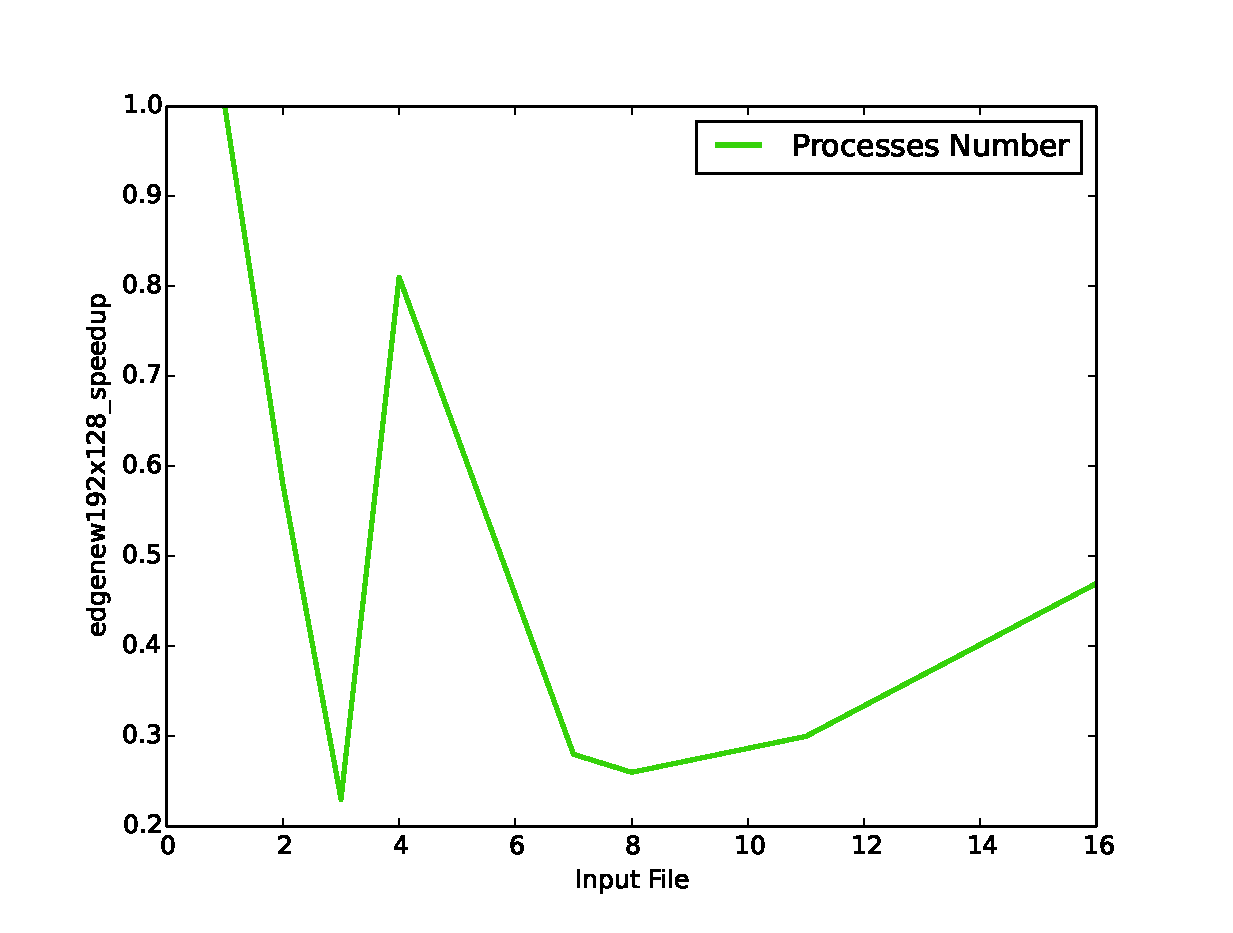
\includegraphics[scale=0.6]{../graphs/edgenew192x128_speedup.eps}
                \caption{Running Time Loop 2 with 4 Threads}
                \label{loop2-threads4}
            \end{figure}

        \subsubsection{Average Pixel}
            Performance analysis for the average pixel results.

\sectionVspacing

\section{Conclusion}
In conclusion.

\end{document}

% \begin{table}[h]
% 	\begin{center}
% 		\begin{tabular}{||l|c|l||}
% 			\hline
% 			{\bf Loop No} & {\bf Schedule}\\
% 			\hline
% 			Loop 1         &  schedule(guided, 4)\\
% 			Loop 2         &  schedule(dynamic, 16)\\
% 			\hline
% 		\end{tabular}
% 	\end{center}
% 	\caption{Best scheduler options on four (4) threads}
% 	\label{simple_table}
% \end{table}

% \lstinputlisting[language=C, firstline=2, lastline=3, caption=loops.c]{../template/loops_parallel-B136013.c}
